\section{实验设置与结果}
\subsection{设置与评价}
正式主方案使用 \texttt{sample\_model.json} 和由 mock trace 变体构成的平衡轨迹，Cube 配置为 $N=3,D=2,H=W=4096$，最大并行 Sub-Cube 数为 9，并启用严格容量比 2.0。主方案使用 V5 参数卡中记录的重叠、搜索、复制、压缩和放置参数；所有输出由 \texttt{validate\_submission.py} 再次检查。评价指标包括端到端延迟、空间利用率、时间利用率、切换代价、冲突分数、映射率和容量比。

\subsection{主方案结果}
表~\ref{tab:primary} 给出 V5 primary 与 First Fit 基线的对比。优化方案将延迟降低 \PrimaryImprovement{}，同时将时间利用率由 0.2355 提升至 \PrimaryTemporal{}，切换代价从 15,576 降至 1,083 cycles。两者映射率均为 1.0。容量比 \PrimaryCapacity{} 小于严格上限 2.0，独立验证报告为 \texttt{ok=true} 且无错误。

\begin{table*}[t]
\centering
\caption{V5 primary 在平衡 mock trace 上的主结果。}
\label{tab:primary}
\begin{tabular}{lrrrrrr}
\toprule
方案 & 延迟(cycles) & 空间利用率 & 时间利用率 & 切换代价 & 冲突分数 & 映射率\\
\midrule
First Fit 基线 & 539,729 & 0.5035 & 0.2355 & 15,576 & 6.0 & 1.0\\
V5 primary & \PrimaryLatency{} & \PrimarySpace{} & \PrimaryTemporal{} & 1,083 & \PrimaryConflict{} & 1.0\\
\bottomrule
\end{tabular}
\end{table*}

\begin{figure*}[t]
\centering
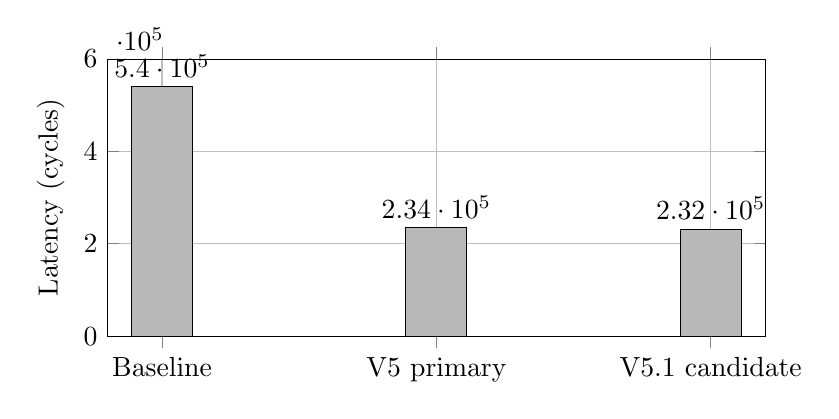
\begin{tikzpicture}
\begin{axis}[
width=.82\textwidth,height=5.1cm,
ybar,bar width=22pt,
symbolic x coords={Baseline,V5 primary,V5.1 candidate},
xtick=data,ylabel={Latency (cycles)},
nodes near coords, nodes near coords align={vertical},
ymin=0,ymax=600000,
grid=major,
]
\addplot[fill=gray!55] coordinates {(Baseline,539729) (V5 primary,234436) (V5.1 candidate,231672)};
\end{axis}
\end{tikzpicture}
\caption{同一平衡 mock trace 上的延迟对比。V5.1 仅为候选，尚需官方激活轨迹复核。}
\label{fig:latency}
\end{figure*}

\subsection{复制消融与候选比较}
在 V5 primary 的消融中，关闭复制后，优化延迟为 257,743 cycles，较基线降低 52.25\%；完整配置为 \PrimaryLatency{} cycles。这表明在该工作负载和参数设置下，副本预算对减少排队与气泡具有贡献。需要注意，当前 Best Fit 加 replication 消融与完整方案在该样例上得到相同延迟，因此该组结果不能单独证明互斥分组带来的边际收益；后续应补充 Best Fit only、分组 only、副本 only 与完整方案的正交消融。

V5.1 将专家副本预算提高至 0.35，同时关闭 shared/non-expert operator replication。它得到 \CandidateLatency{} cycles（\CandidateImprovement{}），较 V5 primary 低 2,764 cycles，但空间利用率升至 \CandidateSpace{}，冲突分数升至 \CandidateConflict{}。因此本文将其表述为 \candidate{}，不替代正式 V5 primary。

\subsection{大规模 metadata-only 验证}
为验证工程链路在较多专家下仍能运行，使用脚本生成 \LargeExperts{} 专家、256 条推理、top-$k=4$ 的 metadata-only MoE 模型与轨迹，并采用 $N=3,D=8,H=W=4096$。优化后延迟由 175,720 降至 \LargeLatency{} cycles，降低 \LargeImprovement{}，映射率为 1.0，容量比为 1.9427。该实验只证明 parser、映射、调度与验证器在更大专家数量下可运行；它不等价于真实 DeepSeek-671B 权重部署或官方轨迹性能。

\subsection{局限性与可复现性}
截至本文完成时，正式评测激活轨迹尚未在本地项目中完成回归，因而所有性能数字受 mock/synthetic trace 分布约束。部分硬件惩罚参数为调度模型假设，未由芯片实测校准。ONNX 支持是元数据级轻量适配，未覆盖完整执行语义。尽管存在这些边界，项目保存了输入哈希、配置、映射、调度、内部 IR、可视化和验证报告；在当前代码版本上，项目虚拟环境回归测试记录为 \TestCount{} passed。
